\documentclass[a4paper,11pt]{article}
\usepackage[utf8]{inputenc}
\usepackage{graphicx}
\usepackage{fullpage}
\renewcommand{\figurename}{Imagem}

\author{André Melo (75882) e Rui Marques (75969)}
\title{Movimento de uma carga eléctrica entre três cargas fixas}
\date{13 de Janeiro de 2013}


\begin {document}
\maketitle
\section{Introdução}
O presente programa pretende simular graficamente o movimento de uma carga eléctrica $q_{0}$ quando sujeita ao campo eléctrico de três outras cargas fixas ($Q_{1},Q_{2},Q_{3}$)). O utilizador pode regular as características das cargas,  nomeadamente o  seu valor, posição e massa. No caso da carga livre, em vez do raio, pode regular-se a massa; é ainda possivel conferir-lhe uma velocidade inicial. De modo a evitar que se gerassem forças de ordem de grandeza muito elevada, considerou-se que, quando as cargas se sobrepõe, a força eléctrica é nula.
\section{Método}
A equação que rege o problema é a Lei de Coulomb, que é dada por:
\begin{equation}
\mathbf{\vec{F}_{0,i}} = k_{e}\frac{q_{0}Q_{i}\vec{e_{r}}}{r^{2}_{0.i}}=q_{0}\vec{E_{i}}, i\in{1,2,3}
\end{equation}


O programa foi escrito em C, sendo que a interface gráfica foi concebida em \textsc{GTK+} e \textsc{Cairo}. O \textsc{GTK+} foi instrumental no desenvolvimento do ambiente de janela do programa, enquanto que o \textsc{Cairo} foi utilizado para gerar o movimento das cargas no ecrã.
O código do programa está divido em diferentes ficheiros, nomeadamente:
\begin{enumerate}
\item \emph{cargas.c}, onde está programada a interface gráfica: o ambiente de janelas, o movimento das cargas, as funções \emph{callback}, entre outros.
\item \emph{electric.h/electric.c}, onde estão definidas a estrutura de uma carga (\emph{charge}) e o calculo do campo $\vec{E_{q_{0}}}$ respeitantes às mesmas.
\item \emph{vector.h/vector.c}, onde estão definidas as operações relativas ao calculo vectorial.
\end{enumerate}


O problema em causa implica a resolução de uma equação diferencial de $2^{a}$ ordem, que foi tratada computacionalmente recorrendo ao método de \textsc{Euler-Crommer}. Praticamente todos os cálculos foram feitos vectorialmente (com coordenadas cartesianas). A função \emph{coulomb} permite o cálculo do campo entre $q_{0}$ e $Q_{i}$, e a função \emph{eletric} soma vectorialmente todos os campos elétricos. Com estes dados, basta calcular a força/aceleração e aplicar o metodo \textsc{Euler-Crommer}. Como o \emph{refresh rate} do ecran é relativamente lento para permitir cálculos exactos usando este método, a solução encontrada foi fazer um 1000 ciclos a cada refresh do ecrã, apurando os cálculos sem comprometer a componente gráfica. Sendo o \emph{refresh rate} de $10^{-2}$ s, e o numero de ciclos em cada \emph{refresh} de 1000, o intervalo de tempo "infinitesimal" dt será $10^{-5}$, garantindo assim o tempo real.


O diminsionamento de velocidades iniciais, massas e raios foi o necessário de modo a que haja um movimento de ordem de velocidade aceitável ao olho humano e às capacidades gráficas de um computador modesto, tendo ainda em conta que o valor de cada carga pode estar no intevalo [-50,50]. A constante \emph{k} foi assim definida em $10^{6}$, como \emph{macro} no ficheiro \emph{eletric.h}.


A cronometragem do tempo foi feita com a função \emph{clock()} do \emph{time.h} pois assegura um controlo do tempo mais fidedigno. Esse tempo é o tempo usado para a geração de gráficos. Os gráficos e o rasto são feitos tendo em conta os ultimos 400 pontos. Os gráficos têm reajustamento automatico mas caso o utilizador queira, pode alterar a escala (não aconselhavel).
\section{Explicação da interface do programa}
Apresenta-se, abaixo, uma imagem do programa.
\begin{figure}[h!]
\centering
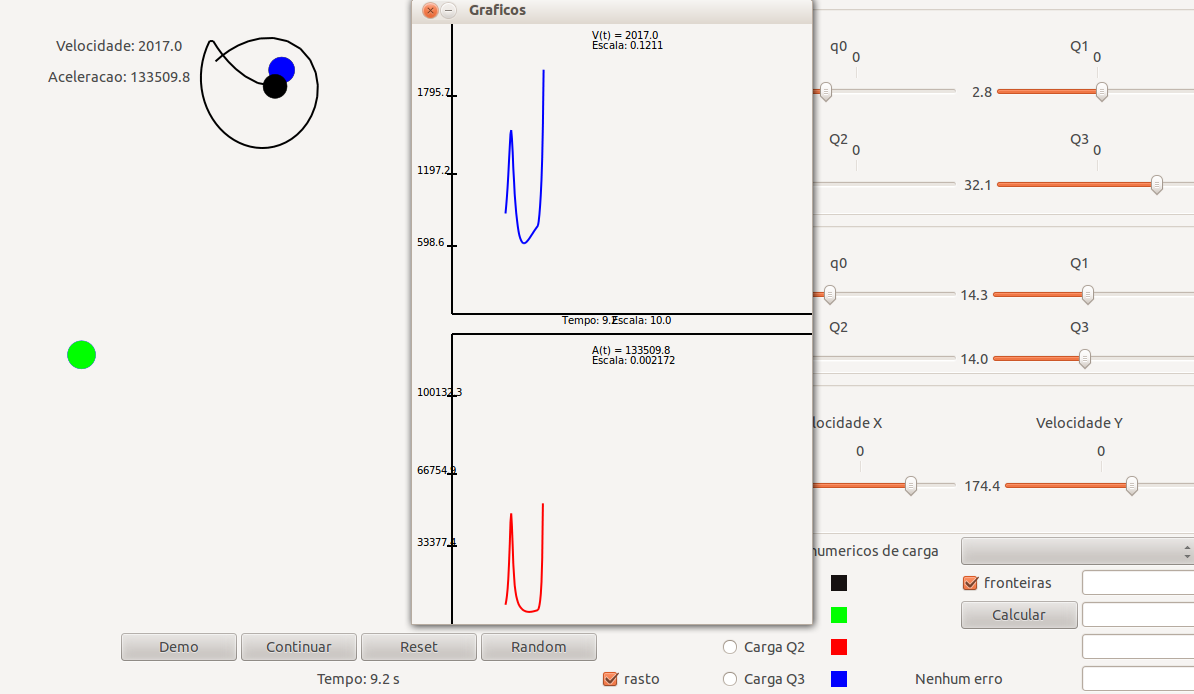
\includegraphics[scale=0.25]{screenshot.png}
\caption{\emph{Screenshot} do programa}
\end{figure}


Na secção à esquerda, encontra-se a simulação pretendida, bem como botões "Iniciar/Pausa", \emph{Reset}, \emph{Demo} (introduz valores para uma demonstração) e \emph{Random} (gera uma configuração aleatória de cargas, quer em posição, velocidade, massa e carga) que permitem ao utilizador controlar o decurso da simulação. Existe tambem uma \emph{checkbox} que desactiva ou activa o rasto da trajectória da bola e outro que permite controlar a existência de fronteiras.


Já à direita, encontram-se os controlos que dizem respeito às cargas. O utilizador pode, deste modo, regular as caracteristicas das cargas em tempo real, recorrendo aos \emph{sliders}. Para alterar a posição das cargas, deve seleccionar-se, no conjuto de \emph{radio buttons} do canto inferior direito, a carga alterar e, seguidamente, clicar no local onde se deseja fixar a mesma. À direita dos \emph{radio buttons}, o utilizador dispõe de uma \emph{dropdown} e um conjunto de \emph{text fields} que lhe permitem escolher valores de forma mais exacta para as características das cargas e, assim, poder estudar a simulação com maior detalhe.Para isso é necessário introduzir os 4 valores nos campos de escrita, no qual a sua ordem está de acordo com a legenda à esquerda, e de seguida carregar em calcular.


No menu \emph{Opções}, o utilizador pode ainda abrir uma janela de gráficos que mostra em função do tempo a velocidade (a azul) e a aceleração (a vermelho). Existem ainda duas outras opções ("Guardar estado" e "Recuperar estado") que permitem ao utilizador guardar e repor o estado actual da simulação.

Para alterar a escala dos gráficos, é necessário aceder ao menu de "Opções" na janela principal e seleccionar "Alterar escala". Após a abertura da janela de alteração, a escala é alterada através dos \emph{sliders}. Nota: a posição dos \emph{sliders} é alterada em tempo real, logo o melhor é colocar a animação em pausa durante as alterações.
\end{document}
